%\documentclass[journal, onecolumn, letterpaper]{IEEEtran}
%\documentclass[journal,onecolumn]{IEEEtran}
% \documentclass[conference]{IEEEtran}
\documentclass[a4paper, 12pt, onecolumn,singlespacing]{article}

% The preceding line is only needed to identify funding in the first footnote. If that is unneeded, please comment it out.
\usepackage[level]{fmtcount} % equivalent to \usepackage{nth}
% \include{util}
\usepackage[portuguese, brazil, english]{babel}
\usepackage{multirow}
\usepackage{array} % for defining a new column type
\usepackage{varwidth} %for the varwidth minipage environment
\usepackage[super]{nth}
\usepackage{authblk}
\usepackage{cite}
\usepackage{amsmath,amssymb,amsfonts}
\usepackage{ulem}
\usepackage{graphicx}
% \usepackage{subfig}
\usepackage{textcomp}
\usepackage{xcolor}
\usepackage{mathptmx}
\usepackage[T1]{fontenc}
\usepackage{textcomp}
\usepackage{titlesec}
\usepackage{helvet}
\usepackage{gensymb}
\usepackage{setspace} % espacamento entre linhas
\usepackage{pgfplots}
\usepackage{tikz}
\usepackage{subcaption}
\usepackage{minted}
\usepackage[left=2cm, right=2cm, bottom=2cm, top=2cm]{geometry} 
\usepackage{makecell}
\usepackage{pdfpages}
\usepackage[ISO]{diffcoeff}

\renewcommand\theadalign{bc}
\renewcommand\theadfont{\bfseries}
\renewcommand\theadgape{\Gape[4pt]}
\renewcommand\cellgape{\Gape[4pt]}

%dashed line
\usepackage{booktabs, makecell}
\renewcommand\theadfont{\bfseries}
\renewcommand\theadgape{}
\usepackage{arydshln}
\setlength\dashlinedash{0.2pt}
\setlength\dashlinegap{1.5pt}
\setlength\arrayrulewidth{0.3pt}

% padrao 1.5 de espacamento entre linhas
\setstretch{1.5}

\title{Trabalho 01 - Descargas Negativas Descendentes Nuvem - Solo}

\author[1]{Augusto Mathias Adams}
\affil[1]{augusto.adams@ufpr.br}
\setcounter{Maxaffil}{0}
\renewcommand\Affilfont{\itshape\small}

\begin{document}
	% Seleciona o idioma do documento
	\selectlanguage{brazil}
	
	% título
	\maketitle

	\textit{``An electrically active thundercloud may be regarded as an
	electrostatic generator suspended in an atmosphere of low
	electrical conductivity. It is situated between two concentric
	conductors, namely, the surface of the earth and the
	electrosphere, the latter being the highly conducting layers of the
	atmosphere at altitudes above 50 to 60 km.''} - Malan, 1967

	\section{Resumo do Processo de Descarga}
	
	\textbf{A descarga negativa descendente em direção ao solo é o tipo mais comum e estudado de raios}. Cada \textit{flash} para o solo geralmente contém de três a cinco \textit{strokes}, sendo que o número máximo de \textit{strokes} já observados em um único \textit{flash} é de 26. A maioria esmagadora, com cerca de 80\% ou mais, dos \textit{flashes} contém mais de um \textit{stroke}. O intervalo de tempo entre os sucessivos \textit{strokes} em um \textit{flash} é geralmente de várias dezenas de milissegundos, embora possa ser tão grande quanto centenas de milissegundos se uma corrente contínua longa estiver envolvida ou tão pequeno quanto um milissegundo ou menos. A duração total de um \textit{flash} é tipicamente algumas centenas de milissegundos, e a carga total transferida para o solo é de algumas dezenas de coulombs. Cerca de metade de todos os \textit{flashes} de descargas para o solo criam mais de uma terminação no solo, com a separação espacial entre as terminações do canal podendo chegar a muitos quilômetros. Cada \textit{stroke} é composto por um líder que se move para baixo e um líder que se move para cima no canal de retorno. O líder cria um caminho condutor entre a fonte de carga na nuvem e o solo e deposita carga negativa ao longo desse caminho, enquanto o canal de retorno percorre esse caminho, movendo-se do solo em direção à fonte de carga na nuvem e neutraliza a carga negativa do líder. O líder escalonado inicia os movimentos do primeiro \textit{stroke} de retorno intermitentemente, enquanto os líderes dos \textit{strokes} subsequentes geralmente parecem se mover continuamente\cite{RAKOV_UHMAN}.
	
	Após a quebra inicial, possivelmente entre as principais regiões de carga negativa e positiva inferiores na nuvem, o líder escalonado se propaga em direção ao solo com uma velocidade média de $2 \times 10^{5}$ $\frac{m}{s}$. Abaixo do limite inferior da nuvem, cada passo do líder tem uma duração típica de 1 $\mu s$ e um comprimento de dezenas de metros, com um intervalo de tempo entre os passos de 20 a 50 $\mu s$ . A corrente média do líder escalonado está entre 100 e 1000 $A$, e o valor máximo do pulso de corrente associado a um único passo é de pelo menos 1 $kA$. A transição da fase do líder para a fase do canal de retorno é referida como o processo de anexação. A velocidade de propagação ascendente de um canal de retorno abaixo do limite inferior da nuvem é tipicamente entre um terço e metade da velocidade da luz, ou seja, cerca de três ordens de magnitude mais alta que a velocidade do líder escalonado. A primeira corrente do canal de retorno medida no solo sobe para um pico inicial de cerca de 30 $kA$ (valor mediano) em alguns microssegundos e diminui para metade do valor de pico em algumas dezenas de microssegundos. O canal de retorno descarrega ao solo os vários coulombs de carga originalmente depositados no canal do líder escalonado. A onda de corrente do canal de retorno aquece rapidamente o canal para uma temperatura máxima próxima a 30.000 $K$ e cria uma pressão de canal da ordem de 10 atm ou mais, resultando na expansão do canal, radiação óptica intensa e uma onda de choque acústica que eventualmente se torna o trovão que ouvimos à distância\cite{RAKOV_UHMAN}.
	
	As descargas subsequentes ocorrem após a cessação do fluxo de corrente para o solo. Processos na nuvem chamados de processos J envolvem uma redistribuição de cargas na nuvem em uma escala de tempo de dezenas de milissegundos em resposta ao retorno de curso anterior. Transitórios ocorrendo durante o processo mais lento J são referidos como processos K. Ambos os processos J e K em descargas entre nuvens e o solo efetivamente transportam cargas negativas frescas para dentro e ao longo do canal existente (ou seus remanescentes), embora não até o solo. O líder \textit{dart} progride para baixo a uma velocidade típica de $10^7$ $\frac{m}{s}$ e deposita uma carga total ao longo do canal da ordem de 1 $C$. A corrente de pico do líder \textit{dart} é de cerca de 1 $kA$. A corrente de retorno subsequente medida no solo atinge um valor de pico de 10 a 15 $kA$ em menos de um microssegundo e decai para metade do valor de pico em algumas dezenas de microssegundos. A derivada máxima da corrente é tipicamente da ordem de 100 $\frac{kA}{\mu s}$. A velocidade média de propagação ascendente de cursos de retorno subsequentes é semelhante à dos primeiros cursos de retorno. O componente de canal de retorno de uma corrente de canal de retorno subsequente é frequentemente seguido por uma corrente contínua contínua que tem uma magnitude de dezenas a centenas de amperes e uma duração de até centenas de milissegundos. Os processos transitórios que ocorrem durante o estágio de corrente contínua contínua e servem para transportar carga negativa para o solo são referidos como componentes M. O modo de transferência de carga M para o solo, em oposição ao modo líder-canal de retorno, requer a existência de um canal aterrado transportando corrente\cite{RAKOV_UHMAN}.
	
	\section{Características da Forma De Onda Detectada ($\vec{E}$, $\vec{B}$)}

	\subsection{Introdução}
	
	A forma de onda de campo elétrico típica de um raio é mostrada na figura \ref{initial_breakdown}:
	
	\begin{figure}[!h]
		\centering
		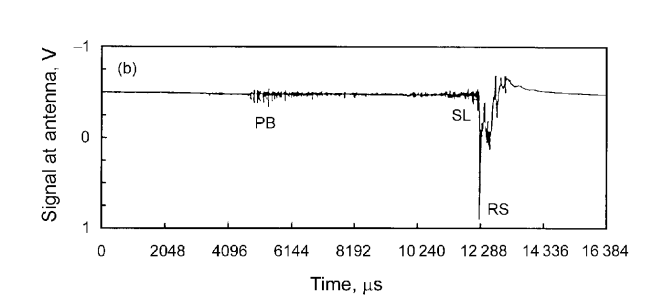
\includegraphics[scale=1.9]{imagens/initial_breakdown.png}
		\caption{Forma de Onda de uma descarga negativa descendente. Em sequência à quebra inicial, há a formação do líder escalonado, o processo de anexação e a descarga de retorno. Fonte: \cite{RAKOV_UHMAN}}
		\label{initial_breakdown}
	\end{figure}
	
	A forma de onda do campo elétrico e magnético associada a uma descarga negativa descendente exibe características distintas ao longo do tempo.
	
	A forma de onda do campo elétrico geralmente começa com um aumento rápido e acentuado durante a fase inicial da descarga. Esse aumento está relacionado à acumulação e liberação de carga elétrica durante o processo de ionização do canal de descarga. O campo elétrico atinge seu valor máximo durante essa fase inicial.
	
	Após o pico inicial, o campo elétrico pode apresentar oscilações menores, conhecidas como "pulsos de campo". Esses pulsos são resultado de reflexões e interações do campo elétrico com a geometria do canal de descarga e as características do ambiente circundante. Essas oscilações podem ser observadas como variações periódicas na forma de onda do campo elétrico.
	
	Quanto ao campo magnético, sua forma de onda está intimamente relacionada à corrente elétrica que flui durante a descarga. Durante a fase inicial da descarga, o campo magnético aumenta rapidamente, acompanhando o aumento do campo elétrico. Esse pico inicial é causado pela corrente elétrica intensa que flui na descarga.
	
	À medida que a descarga progride, o campo magnético também pode apresentar oscilações menores, mas geralmente com menor amplitude do que o campo elétrico. Essas oscilações magnéticas estão associadas às variações na corrente elétrica ao longo do canal de descarga.
	
	À medida que a descarga se aproxima do término, tanto o campo elétrico quanto o campo magnético diminuem gradualmente até retornarem próximos a zero. O decaimento desses campos está relacionado ao esgotamento da carga elétrica disponível e à dissipação da energia ao longo do canal de descarga.
	
	A forma de onda do campo elétrico e magnético da descarga negativa descendente fornece informações valiosas sobre as características da descarga, como sua intensidade, duração e dinâmica. Essas informações são importantes para o estudo e compreensão dos fenômenos de descarga atmosférica, além de serem úteis para aplicações como detecção, monitoramento e proteção contra raios.
	
	\subsection{Descrição detalhada da Forma de Onda Detectada}
	
	\subsubsection{ Quebra Inicial (\textit{``initial breakdown''})}
	
		\textbf{O \textit{initial breakdown}\cite{RAKOV_UHMAN}, ou pré-ionização, refere-se ao processo inicial de ionização do ar que ocorre antes da formação completa da descarga atmosférica.} Durante essa fase, a forma de onda do campo elétrico e magnético pode apresentar características distintas.
		
		No caso do campo elétrico, a forma de onda durante o \textit{initial breakdown} é caracterizada por pulsos de curta duração e alta amplitude. Esses pulsos representam os eventos de ionização localizada que ocorrem à medida que a tensão elétrica aumenta e os caminhos condutivos são estabelecidos no ar. A forma de onda do campo elétrico durante o \textit{initial breakdown} pode ter uma aparência errática ou irregular, com oscilações de alta frequência.
		
		Já o campo magnético durante o \textit{initial breakdown} é geralmente de baixa amplitude e pode ser difícil de ser detectado diretamente. Isso ocorre porque a corrente elétrica associada ao \textit{initial breakdown} é relativamente baixa em comparação com a corrente total da descarga atmosférica. No entanto, medidas indiretas e técnicas de processamento de sinal podem ser usadas para identificar o campo magnético durante essa fase.
		
	\subsubsection{Líder Escalonado (\textit{``Stepped Leader''})}
	
		\textbf{O \textit{stepped leader} é um processo inicial na formação de uma descarga atmosférica, que ocorre antes do retorno do raio principal.} Durante o \textit{stepped leader}, o campo elétrico e magnético exibem características distintas em suas formas de onda.
		
		A forma de onda do campo elétrico do \textit{stepped leader} é caracterizada por pulsos de curta duração e alta amplitude. Esses pulsos representam os avanços sucessivos do canal de descarga, que ocorrem em etapas ou "degraus" em direção ao solo. A forma de onda do campo elétrico geralmente possui uma aparência impulsiva, com pulsos de alta frequência e amplitude variável à medida que o \textit{stepped leader} avança.
		
		Já o campo magnético associado ao \textit{stepped leader} é relativamente fraco em comparação ao campo elétrico. A forma de onda do campo magnético é tipicamente de baixa amplitude e pode ser difícil de ser detectada diretamente, especialmente a longas distâncias. No entanto, equipamentos de medição sensíveis e técnicas de processamento de sinal podem ser utilizados para registrar e analisar o campo magnético durante o \textit{stepped leader}.
		
	\subsubsection{Processo de Conexão (\textit{``Attachment Process''})}
	
		\textbf{O \textit{Attachment Process} (processo de conexão) é um estágio crucial durante a formação de uma descarga atmosférica, no qual a corrente elétrica do raio se conecta ao objeto condutor na superfície da Terra}. Durante esse processo, o campo elétrico e magnético exibem características distintas em suas formas de onda.
		
		A forma de onda do campo elétrico durante o \textit{Attachment Process} é caracterizada por pulsos de curta duração e alta amplitude. Esses pulsos representam a transferência rápida de carga elétrica do raio para o objeto condutor, resultando em variações abruptas do campo elétrico próximo à área de anexação. A forma de onda do campo elétrico geralmente mostra uma alta taxa de variação, indicando a intensidade da transferência de carga elétrica durante o \textit{Attachment Process}.
		
		O campo magnético associado ao \textit{Attachment Process} também exibe uma forma de onda distintiva. Geralmente, a forma de onda do campo magnético é caracterizada por pulsos de curta duração e baixa amplitude em comparação ao campo elétrico. A variação do campo magnético está diretamente relacionada à corrente elétrica que flui durante o processo de anexação.
	
	\subsubsection{Descarga de Retorno (\textit{``Return Stroke''})}
		\textbf{O \textit{Return Stroke} (descarga de retorno) é o estágio mais significativo e visível de uma descarga atmosférica, onde a corrente elétrica flui rapidamente em direção à nuvem após a conexão com o objeto condutor na superfície da Terra}. Durante esse processo, o campo elétrico e magnético exibem características distintas em suas formas de onda.
		
		A forma de onda do campo elétrico do \textit{Return Stroke} é caracterizada por um pulso inicial de alta amplitude e curta duração, seguido por uma queda exponencial gradual. O pulso inicial, também conhecido como pulso de pico, é gerado pela rápida transferência de carga elétrica da nuvem para o solo. Em seguida, o campo elétrico diminui gradualmente em magnitude à medida que a corrente elétrica se estabiliza.
		
		O campo magnético associado ao \textit{Return Stroke} também possui uma forma de onda distinta. Sua forma de onda geralmente segue um padrão semelhante ao campo elétrico, com um pulso inicial de alta amplitude e uma queda exponencial gradual. A variação do campo magnético está diretamente relacionada à variação da corrente elétrica durante o retorno do golpe.
		
		A forma de onda do campo elétrico e magnético do \textit{Return Stroke} é caracterizada por sua rápida variação e magnitude significativa. Essas características são responsáveis pela emissão de radiação eletromagnética associada aos raios, que podem ser detectadas e medidas por equipamentos apropriados.
	
	\subsubsection{Líder \textit{``Dart''}}
	
		\textbf{O \textit{``Dart Leader''}, ao contrário de um \textit{``Stepped Leader''} parece se mover continuamente, ou seja, a porção mais baixa do canal do líder, chamada de \textit{``dart''}, permanece luminosa durante a extensão do canal da nuvem para o solo}. Muitas descargas subsequentes (mais de um terço dos segundos \textit{return strokes} em canais não muito antigos) são iniciados por líderes que exibem degraus pronunciados na porção inferior do canal. Esses líderes produzem sequências regulares de pulsos que são observadas logo antes do pulso do retorno em registros de campo elétrico ou magnético distantes e são chamados de líderes \textit{dart} em degraus.
	
	\subsubsection{Corrente Contínua}
	
		\textbf{A corrente contínua, também conhecida como "\textit{continuing current}" em inglês, é geralmente definida como a corrente de baixo nível que segue imediatamente um descarga de retorno (\textit{return stroke}) em uma mesma trajetória em direção ao solo.} Essa corrente geralmente possui valores de dezenas a centenas de amperes e dura entre dezenas a centenas de milissegundos. Essa corrente pode ser vista como um arco quase estacionário entre a fonte de carga na nuvem e o solo ao longo do caminho criado pela sequência ou sequências anteriores de líder e retorno de corrente.
		
		A forma de onda da corrente contínua geralmente exibe um perfil característico, com uma amplitude relativamente constante e uma duração prolongada. Inicialmente, após o retorno de corrente, a corrente aumenta rapidamente até atingir seu valor máximo. Em seguida, ela se estabiliza em um nível mais baixo e mantém-se relativamente constante ao longo do tempo. 
	
	\subsubsection{Componente M}
		\paragraph{Componente M}
		As componentes M são perturbações na corrente de relâmpagos de variação lenta, acompanhadas por aumentos na luminosidade do canal de relâmpagos. Inicialmente, Malan e Collens (1937) relataram, a partir de registros ópticos em tempo real de relâmpagos naturais, que as componentes M são aumentos transitórios de luminosidade em canais de relâmpagos pouco luminosos e aterrados abaixo da base da nuvem. As características das formas de onda da corrente das componentes M foram primeiramente descritas por Thottappillil et al. (1995), em relâmpagos provocados por foguete. Eles descobriram que o tempo de subida de 10\% a 90\% da corrente da componente M varia de dezenas de microssegundos a milissegundos, com uma média geométrica de 422 $\mu$s. As magnitudes da corrente da componente M variam de dezenas de amperes a alguns quiloamperes, com uma média geométrica de 117 A. A pressão de pico dos sinais acústicos das componentes M está na mesma ordem de grandeza da sequência líder/descarga de retorno (Rakov \& Uman, 2003, Capítulo 4). As componentes M podem ser as principais responsáveis pelos chamados sprites atrasados, que ocorrem dezenas de milissegundos após a descarga de retorno (por exemplo, Li et al., 2008; Yashunin et al., 2007).
	
		Rakov et al. (1992), a partir da análise de registros de campo elétrico de relâmpagos nuvem-solo a distâncias que variam de 2,5 a 27 km na Flórida, relataram que mais da metade das formas de onda do campo elétrico das componentes M estão associadas a pulsos de campo elétrico em microssegundos. Na maioria dos casos, esses pulsos ocorrem no início das formas de onda do campo elétrico em formato de gancho das componentes M. Shao et al. (1995), que utilizaram um interferômetro de frequência muito alta (VHF) de banda estreita, descobriram que a iniciação das componentes M está geralmente associada ao desenvolvimento de um canal dentro da nuvem que se conecta ao canal que transporta a corrente contínua (CC) em direção ao solo. Observações semelhantes para pulsos de corrente contínua inicial (ICC) e componentes M em relâmpagos provocados por foguete foram relatadas por Yoshida et al. (2012) e Pilkey et al. (2013), respectivamente, por meio da imagem VHF de canais de relâmpagos usando um interferômetro VHF de banda larga e uma Matriz de Mapeamento de Relâmpagos.
		
		Um exemplo de assinatura do campo elétrico em formato de gancho característica da componente M é encontrado na Figura \ref{componente_m}. Tran et al. (2013), que analisaram formas de onda do campo elétrico registradas a 45 km do canal de raios provocados por foguete, relataram que as componentes M pronunciadas nos registros de corrente na base do canal são frequentemente precedidas por pulsos de campo em microssegundos (característica relatada inicialmente por Rakov et al., 2001). Acredita-se que esses pulsos sejam produzidos pela intercepção de líderes dentro da nuvem pelo canal aterrado que transporta a corrente. Durante a fase inicial de raios provocados por foguete e de relâmpagos ascendentes iniciados por torres, alguns (se não a maioria) dos chamados pulsos de corrente contínua inicial (ICC) exibem muitas semelhanças com as "clássicas" componentes M que ocorrem durante a corrente contínua após a descarga de retorno.
		
			\begin{figure}[!htb]
				\caption{(a) Corrente, (b) campo magnético e (c) campo elétrico para um grande componente M que seguiu o segundo golpe de um relâmpago disparado por foguete em Camp Blanding, Flórida. Os campos foram registrados a uma distância de 280 m do canal de iluminação. Observe que o pico do campo elétrico ocorre significativamente antes dos picos de corrente e campo magnético. Adaptado de Rakov et al. (1998).}
				\label{componente_m}
				\subfloat[\label{componente_m_a}]{
						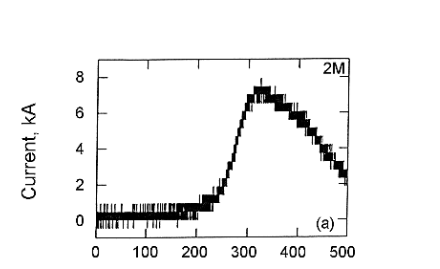
\includegraphics[width=0.32\textwidth]{imagens/componente_m_a.png}
					} \hfill
				\subfloat[\label{componente_m_b}]{
						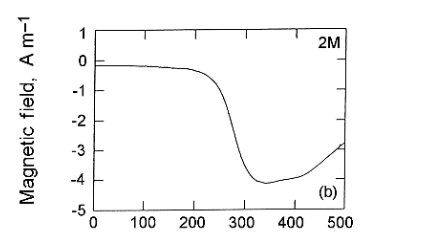
\includegraphics[width=0.32\textwidth]{imagens/componente_m_b.png}
					}
				\subfloat[\label{componente_m_c}]{
						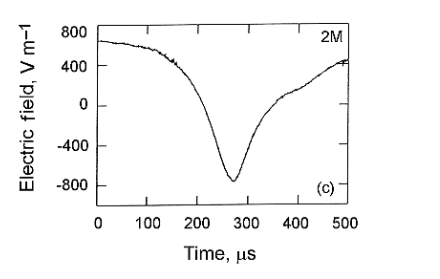
\includegraphics[width=0.32\textwidth]{imagens/componente_m_c.png}
					}
			\end{figure}
		\paragraph{Trem de Pulsos Regulares (\textit{Regular Pulse Bursts})}
		
		Um trem de pulsos regulares em uma descarga atmosférica geralmente está associado ao fenômeno conhecido como \textit{Componente M}. O campo eletromagnético de um trem de pulsos regulares é caracterizado por variações rápidas e repetitivas na intensidade do campo elétrico e magnético ao longo do tempo.
		
		Durante a ocorrência da componente M, são observadas oscilações de alta frequência (geralmente na faixa de 3 a 300 MHz) no campo elétrico e magnético. Essas oscilações têm amplitudes significativamente maiores do que as encontradas em outras descargas intra-nuvem ou nuvem-solo típicas.
		
		O campo elétrico de um trem de pulsos regulares geralmente é registrado como uma série de pulsos bipolares com uma duração total de cerca de 10 a 20 microssegundos. A amplitude desses pulsos bipolares é aproximadamente um terço do valor máximo do campo elétrico observado durante um retorno típico de um raio.
		
		É importante mencionar que, durante o trem de pulsos regulares, a polaridade dos pulsos bipolares é oposta à polaridade dos campos elétricos observados em descargas nuvem-solo negativas durante condições meteorológicas normais. Isso significa que, na primeira metade do pulso bipolar, a direção do campo elétrico é oposta à direção do campo elétrico de tempo bom. Essa inversão de polaridade é uma característica distintiva da componente M.
		
		Portanto, o campo eletromagnético de um trem de pulsos regulares em uma descarga atmosférica, como o M-componente, exibe variações rápidas e repetitivas no campo elétrico e magnético, com polaridade inversa em relação ao campo elétrico de tempo bom.


	\subsubsection{Processos J e K}
	
		\paragraph{Processo J} O processo J \cite{UHMAN_1987}, ou "junção", ocorre na nuvem durante o intervalo de tempo entre os \textit{Return Strokes}. Ele é identificado com um campo elétrico que apresenta uma mudança relativamente constante em uma escala de tempo de dezenas de milissegundos. A mudança J pode ser positiva ou negativa, geralmente é menor do que a mudança do campo devido à corrente contínua e, ao contrário da mudança do campo de corrente contínua, não está associada a um canal luminoso entre a nuvem e o solo. Pequenas variações relativamente rápidas do campo elétrico, chamadas de mudanças K, também ocorrem entre os golpes geralmente em intervalos de 2-20 milissegundos, e parecem estar superpostas à mudança geral do campo elétrico associada ao processo J.
		
		Há controvérsias em relação à interpretação física da mudança do campo entre os golpes associada ao processo "junção": a maioria dos pesquisadores associa a mudança do campo J a uma descarga na nuvem que disponibiliza carga para o topo do canal do golpe anterior, a fim de iniciar um líder de dardo, enquanto alguns indicam que o processo J pode ser independente da fonte de carga do líder \textit{dart} e estar relacionado à remoção de carga de centros de carga envolvidos com \textit{strokes} anteriores.
		
		
		\paragraph{Processo K}
		
		O processo K \cite{UHMAN_1987} é geralmente visto como um "líder de recuo" ou um pequeno \textit{return stroke} que ocorre quando uma descarga em propagação dentro da nuvem encontra um centro de carga oposta à sua própria (Ogawa e Brook, 1964). Nessa visão, o processo J representa uma descarga de propagação lenta que inicia o processo K. Ogawa e Brook (1964) forneceram evidências a partir de medições do campo elétrico e fotográficas em raios de luz que comprovam esse caso para as mudanças K em descargas dentro da nuvem. É razoável esperar que as mudanças K nas descargas dentro da nuvem sejam semelhantes às mudanças K na parte dentro da nuvem das descargas para o solo, especialmente considerando que a distribuição dos intervalos de tempo entre as mudanças K foi encontrada por Kitagawa e Brook (1960) para ser quase idêntica tanto para descargas dentro da nuvem quanto para descargas para o solo.
		
		Brook e Vonnegut (1960) e Kitagawa e Brook (1960) sugerem que a mudança lenta do campo J pode ser interpretada como devida à integração temporal instrumental de uma série de pequenas mudanças rápidas do campo K, com duração inferior a 1 milissegundo e mudança de momento entre algumas centenas e 1 $C-km$. Nessa visão, a mudança J é o traço suavizado do registro do campo elétrico, que na realidade consiste em um número de pequenos passos de mudança K. Ogawa e Brook (1964) afirmam que os passos associados aos processos K observados em curta distância constituem a maior contribuição para a mudança geral do campo na última fase de uma descarga dentro da nuvem. Não está claro por que o processo K deve produzir uma mudança significativa no campo, enquanto a descarga de propagação lenta que o inicia não produz, exceto talvez pelo fato de que a mudança K move uma carga relativamente grande a uma distância relativamente longa em comparação com o movimento de carga equivalente no tempo entre as mudanças K. É interessante notar que aparentemente outra visão do processo K foi sugerida por Kitagawa et al. (1962), que argumentam que a mudança K "é evidência do movimento de líderes penetrantes em regiões frescas da nuvem, líderes cuja ocorrência deve ser determinada inteiramente pelas condições dentro da nuvem".
		
		A figura \ref{process_J_K_M} mostra as mudanças de campo elétrico durante um processo de descarga de retorno, onde os processos J e K, além de componentes M, aparecem claramente em ordem cronológica:
		
		\begin{figure}[!h]
			\centering
			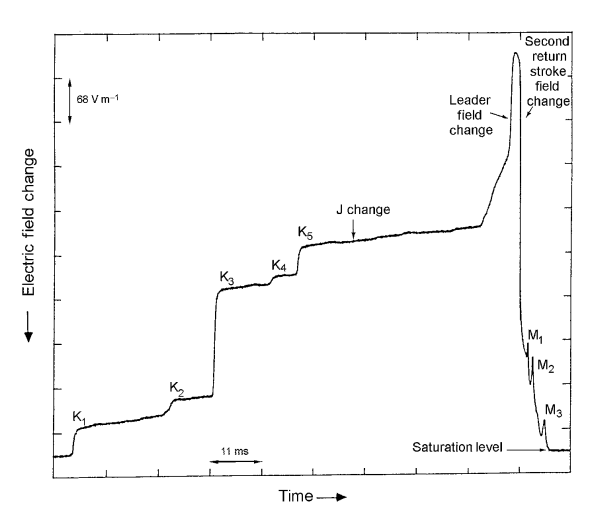
\includegraphics[scale=1.9]{imagens/process_J_K_EFIELD.png}
			\caption{Uma parte do registro do campo elétrico para um relâmpago que ocorreu na Flórida em 1979 às 22h28min43s (UTC) a uma distância de 2,5 km. São identificadas cinco mudanças K pronunciadas (K1 a K5), uma mudança J, mudanças de campo de líder e golpe de retorno, e três mudanças de campo devido a componentes M (M1 a M3). Uma mudança de campo positiva (convenção de eletricidade atmosférica) se desvia para baixo. Adaptado de \textit{Thottappillil et al. (1990)}. Fonte: \cite{RAKOV_UHMAN}}
			\label{process_J_K_M}
		\end{figure}
		
	
	\section{Descrição do Modelo de Campo $\vec{E}$ e $\vec{B}$ (Thottappillil, 1997)}
	
	Para derivar uma expressão aproximada para o campo elétrico, vamos começar com a expressão geral para o campo eletrostático, conforme apresentado por Thottappillil et al. (1997):
	\begin{equation}
		E_z(r, t) = \frac{1}{2 \pi \epsilon_0} \int_{h(t)}^{H_m} \frac{z'}{R^3(z')} \rho_l \left(z't - \frac{R(z')}{c}\right) dz' - \frac{1}{2 \pi \epsilon_0} \frac{H_m}{R^3(H_m)} \int_{h(t)}^{H_m} \rho_l \left(z't - \frac{R(z')}{c}\right) dz'
		\label{eq_E_geral}
	\end{equation}

	onde $R(H_m) = \sqrt{(H_m^2 + r^2)}$  e $h(t)$ é a altura em que o observador "vê" a extremidade inferior do canal do líder; $h(t)$ é determinado pela solução de $t = \frac{H_m - h(t)}{\upsilon} + \frac{\sqrt{h^2(t) + r^2}}{c}$.
	
	O primeiro termo da equação \ref{eq_E_geral} representa a variação do campo devido à carga no canal do líder que se estende para baixo, e o segundo termo representa a variação do campo devido ao esgotamento da carga na fonte de carga da nuvem, à medida que ela é "drenada" pelo canal do líder em expansão. A carga total no canal do líder em qualquer momento é igual à carga total removida da fonte de carga da nuvem, de modo que a carga líquida no sistema canal-fonte global é zero em todos os momentos.
	
	Assumindo que a diferença máxima no tempo de propagação de qualquer fonte no canal até o observador é muito menor do que o tempo necessário para variações significativas nas fontes (ou seja, os efeitos de retardamento são negligenciáveis), e reescrevendo a equação \ref{eq_E_geral} como:
	
	\begin{equation}
		E_z(r, t) = -\frac{1}{2 \pi \epsilon_0} \int_{h(t)}^{z_t} \left[\frac{z'}{R^3(z')} - \frac{H_m}{R^3(H_m)}\right] \rho_L(z', t) dz'
		\label{eq_E_mod_1}
	\end{equation}
	
	onde $z_t = H_m - \upsilon t$ é a altura da ponta do líder no tempo $t$ e $\upsilon$ é a velocidade do líder, assumida como constante.
	
	Assumindo que $\rho_L (z', t) = \rho_L = constante$, o que corresponde a um canal líder uniformemente carregado, pode-se reescrever a equação \ref{eq_E_mod_1} da seguinte forma:
	
	\begin{equation}
		E_z(r,t) = \frac{\rho_L}{2 \pi \epsilon_0 r} \left[\frac{1}{\sqrt{1 + \left(\frac{z_t}{r}\right) ^2}} - \frac{1}{\sqrt{1 + \left(\frac{H_m}{r}\right) ^2}} - \frac{\left(H_m - z_t\right) H_m}{r^2\sqrt{1 + \left(\frac{z_t}{r}\right) ^2}}\right]
		\label{eq_E_mod_2}
	\end{equation}
	
	Para um ponto de campo muito próximo, onde $H_m \geq 2r$, e para $z_t = 0$ (líder tocando o solo) ou $z_t \geq r^2$ e $z_t \geq H_m$ (líder próximo ao solo), a equação \ref{eq_E_mod_2} é aproximada por:
	
	\begin{equation}
		E_z(z_t = 0) \approx \frac{\rho_L}{2 \pi \epsilon_0 r}
		\label{eq_E_mod_3}
	\end{equation}
	
	Ou seja, muito próximo ao canal, a variação vertical do campo eletrostático no solo devido ao canal do líder totalmente desenvolvido diminui com a distância como $r^-1$, ao contrário da variação $r^-3$ longe do canal ($Hm^2 \leqq r^2$). Curiosamente, a equação \ref{eq_E_mod_3} é exatamente a mesma expressão do campo radial produzido por uma carga linear infinitamente longa e uniforme no espaço livre.
	
	A aproximação magnetostática para os campos magnéticos do líder geralmente é escrita em termos da corrente $I(t)$, que se supõe variar lentamente e ser a mesma em todas as alturas ao longo do canal vertical de relâmpago (por exemplo, Uman 1987, 2001). Uma formulação menos familiar, em termos da densidade de carga $\rho_L$, para o campo magnético do líder foi dada por Thottappillil et al. (1997). O campo magnetostático de um canal vertical de líder, cuja extremidade superior está a uma altura Hm e a extremidade inferior a uma altura $z_t = h(t)$ , é dado por:
	
	\begin{equation}
		B_\phi(r, t) = \frac{\mu_0}{2  \pi r} \left[\frac{H_m}{R(H_m)} - \frac{z_t}{R(z_t)}\right]I(t)
		\label{eq_B_mod_1}
	\end{equation}

	Para um canal totalmente desenvolvido, isto é, $z_t = 0$, a equação \eqref{eq_B_mod_1} se torna:
	
	\begin{equation}
		B_\phi(r, t) = \frac{\mu_0}{2  \pi r}\left[\frac{H_m}{R(H_m)}\right]I(t)
		\label{eq_B_mod_2}
	\end{equation}

	A Equação \ref{eq_B_mod_2} é a expressão para o campo magnetostático de uma linha vertical de corrente, cuja extremidade inferior está no solo (um condutor perfeito) e a extremidade superior está a uma altura $H_m$. Se o ponto de observação estiver muito próximo à base do canal, de modo que $r < H_m$, a Equação \ref{eq_B_mod_2} pode ser ainda mais simplificada para obter:
	
	\begin{equation}
		B_\phi(r, t) = \frac{\mu_0  I(t)}{2  \pi r}
	\end{equation}

	que é a mesma equação de uma linha de corrente infinitamente longa no espaço livre.

	
	\section{O que é radiação "\textit{Narrowband}"}
	
		\paragraph{Definição} A radiação \textit{Narrowband} das descargas atmosféricas refere-se à emissão de ondas eletromagnéticas em uma faixa de frequência estreita durante o processo de uma descarga atmosférica, como um raio. Durante uma descarga atmosférica, os elétrons são acelerados a altas velocidades devido à intensa energia elétrica envolvida, o que resulta na emissão de radiação eletromagnética.
		
		A característica distintiva da radiação \textit{Narrowband} é sua largura de banda estreita, o que significa que as ondas eletromagnéticas são emitidas em frequências específicas e bem definidas. Essas frequências geralmente estão na faixa de rádio, abrangendo desde algumas centenas de kilohertz até algumas dezenas de megahertz.
		
		A radiação \textit{Narrowband} das descargas atmosféricas é resultado das oscilações dos elétrons durante o processo da descarga. Essas oscilações geram campos elétricos e magnéticos que se propagam como ondas eletromagnéticas. Essas ondas podem ser detectadas e medidas utilizando equipamentos especializados.
		
		A análise da radiação \textit{Narrowband} das descargas atmosféricas é importante para compreender os processos físicos envolvidos nas descargas elétricas, como a dinâmica das correntes elétricas e a geometria do canal de descarga, entre outros aspectos relevantes. Além disso, a radiação \textit{Narrowband} pode ser utilizada em aplicações como detecção e monitoramento de raios, bem como em pesquisas científicas relacionadas ao clima e à atmosfera terrestre.
		
		Embora as frequências mais comuns da radiação \textit{Narrowband} em descargas atmosféricas estejam na faixa de rádio, é importante destacar que essa radiação não se limita apenas a essas faixas de frequência. Ela pode ocorrer em frequências mais altas ou mais baixas, dependendo das condições específicas da descarga.
		
		Além da radiação \textit{Narrowband}, as descargas atmosféricas também podem produzir radiação de banda larga, conhecida como "ruído atmosférico", que abrange um espectro mais amplo de frequências. Essa radiação de banda larga pode ser detectada em uma ampla faixa de frequências, desde ondas de rádio até frequências de micro-ondas e além.
		
		Aqui estão alguns exemplos de radiação \textit{Narrowband} emitida por raios:
		\begin{itemize}
			\item \textbf{\textit{Radiação de frequência muito alta (VHF):}} Durante as descargas atmosféricas, pode ocorrer a emissão de radiação de VHF, que abrange a faixa de frequência de aproximadamente 30 MHz a 300 MHz. Essa radiação é considerada narrowband em relação ao espectro eletromagnético geral.
			
			\item \textbf{\textit{Radiação de frequência extremamente baixa (ELF):}} Os raios também podem gerar radiação de ELF, que abrange a faixa de frequência de aproximadamente 3 Hz a 3 kHz. Embora seja uma faixa de frequência relativamente baixa, a radiação de ELF ainda é considerada narrowband em comparação com o espectro eletromagnético mais amplo.
			
			\item \textbf{\textit{Ondas de rádio de frequência muito baixa (VLF):}} As descargas elétricas dos raios podem criar perturbações nas ondas de rádio de VLF, que operam na faixa de frequência de aproximadamente 3 kHz a 30 kHz. Essas perturbações são caracterizadas por uma faixa estreita de frequências e podem ser detectadas por receptores VLF.
			
		\end{itemize}

		Embora os raios sejam conhecidos principalmente por sua radiação de banda larga, eles também podem gerar radiação \textit{Narrowband} em frequências específicas, como VHF, ELF e VLF.
		
		\paragraph{Um exemplo moderno de radiação \textit{Narrowband}} Os resultados da detecção de radiação eletromagnética de descargas elétricas de nuvens com propriedades incomuns foram publicados no início dos anos 80 do século passado\cite{IUDIN_2015}. A principal característica dessas descargas é uma explosão de alta potência de radiação de alta frequência, com frequências de 3 a 300 $MHz$, cujo nível excedia consideravelmente os valores para descargas típicas dentro da nuvem e descargas da nuvem para o solo. Sincronamente com a explosão de radiação de alta frequência, sensores terrestres não calibrados registraram uma variação característica no campo elétrico de baixa frequência na forma de um pulso bipolar com duração total de 10 a 20 $\mu s$ (no experimento, o critério para o início do pulso de campo elétrico foi a superação da intensidade de radiação do nível base, bastante alto, em uma frequência de 3, 139 ou 295 $MHz$). A duração de um pulso bipolar superava em muito a duração do pulso de alta frequência registrado nas proximidades do máximo do pulso de campo elétrico, e a amplitude do pulso bipolar era cerca de $\frac{1}{3}$ do valor de pico do campo elétrico para um \textit{return stroke} típico. Nesse caso, a direção do campo elétrico na primeira metade do período de um pulso bipolar era oposta à direção do campo de tempo bom, ou seja, o pulso bipolar tinha polaridade oposta em comparação com os surtos de campo para a descarga negativa da nuvem para o solo. O fenômeno citado é chamado de Descarga Compacta Intranuvem (\textit{CID}). 
		
	\section{Descrição Gráfica dos Processos $M$, $J$ e $K$}
	
	\paragraph{Processos J e K}
	Os processos J e K são fenômenos elétricos que ocorrem durante descargas atmosféricas, como raios. Eles estão relacionados às variações do campo elétrico entre as diferentes etapas da descarga.
	
	O processo J refere-se a uma mudança relativamente estável no campo elétrico que ocorre durante o intervalo de tempo entre as descargas principais, conhecidas como \textit{``return strokes''}. O campo elétrico durante o processo J pode ter uma mudança positiva ou negativa, e é geralmente menor do que a mudança de campo devido à corrente contínua da descarga principal. Diferente da descarga principal, o processo J não está associado a um canal luminoso entre a nuvem e o solo.
	
	Por outro lado, o processo K envolve variações rápidas e relativamente pequenas no campo elétrico que ocorrem entre as descargas principais, em intervalos de tempo de 2 a 20 milissegundos. Essas variações, conhecidas como \textit{``K-changes''}, são superpostas à mudança geral do campo elétrico associado ao processo J. O processo K é frequentemente interpretado como a ocorrência de pequenas descargas ou \textit{``streamers''} que se movem dentro da nuvem, fornecendo uma contribuição para as variações do campo elétrico entre as descargas principais.
	
	A interpretação exata dos processos J e K e seu papel na dinâmica das descargas atmosféricas ainda é objeto de estudo e debate entre os pesquisadores. Diferentes teorias e observações têm sido propostas para explicar esses processos, e pesquisas adicionais são necessárias para um melhor entendimento de sua natureza e mecanismos subjacentes.
	\pagebreak
	A figura \ref{lightning_process} mostra as etapas de um processo de descarga, visto no espectro óptico:
	
	\begin{figure}[h]
		\centering
		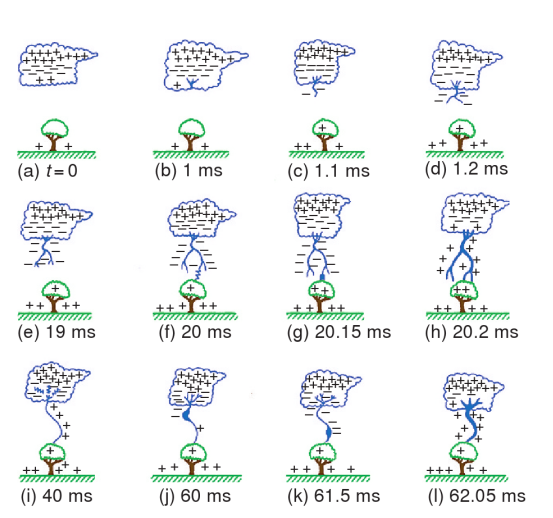
\includegraphics[width=\textwidth]{imagens/lightning_process.png}
		\caption{Esquemático para ilustrar alguns dos processos que levam a um raio no solo que carrega o solo negativamente. (a) Distribuição de carga na nuvem, (b) Quebra Inicial, (c-e) Líder Escalonado, (f) Processo de conexão, (g e h) Primeira descarga de retorno, (i) Processos K e J, (j e k) Líder em dardo e (1) Segunda descarga de retorno. [Adaptado de M. Uman, The Lightning Discharge, Academic Press, Inc., Nova York, 1987, p. 12, Direitos autorais 1987, com permissão da Elsevier.]}
		\label{lightning_process}
	\end{figure}
	
	Etapas explicadas: 
	
	\begin{itemize}
		\item  \textbf{\textit{ (a) Distribuição de carga na nuvem:} }Nesta etapa, a nuvem contém uma separação de cargas positivas e negativas. Tipicamente, a parte inferior da nuvem está carregada negativamente, enquanto a parte superior está carregada positivamente.
		
		\item \textbf{\textit{(b) Quebra Inicial:}} Uma região da nuvem próxima ao solo experimenta um campo elétrico forte, o que leva à iniciação de uma pré-quebra. Esse processo envolve o desenvolvimento de canais de ionização que conectam a nuvem ao solo.
		
		\item \textbf{\textit{(c-e) Líder escalonado:}} O líder escalonado é uma série de canais luminosos e escalonados que se propagam de cima para baixo a partir da nuvem em direção ao solo. Consiste em uma série de descargas rápidas ou degraus, cada uma durando microssegundos. O líder escalonado busca um caminho de menor resistência em direção ao solo, ramificando-se e se estendendo de maneira irregular.
		
		\item \textbf{\textit{(f) Processo de conexão:}} Quando o líder escalonado se aproxima do solo, estabelece-se uma conexão entre ele e um líder invisível em movimento ascendente chamado líder em dardo. Essa conexão é conhecida como processo de conexão.
		
		\item \textbf{\textit{(g e h) Primeira descarga de retorno:}} A primeira descarga de retorno é o canal luminoso principal que transporta a maior parte da corrente do raio do solo para cima. Ocorre após o processo de conexão e se desloca rapidamente ao longo do caminho estabelecido pelo líder escalonado. A primeira descarga de retorno é a parte brilhante e visível do raio.
		
		\item \textbf{\textit{(i) Processos K e J:}} Após a primeira descarga de retorno, pode haver variações no campo elétrico conhecidas como processos K e J. O processo K refere-se a flutuações menores e rápidas no campo elétrico, enquanto o processo J representa uma mudança mais lenta e gradual no campo elétrico.
		
		\item \textbf{\textit{(j e k) Líder \textit{``dart''}:}} Após a primeira descarga de retorno, um novo líder chamado líder \textit{``dart''} se propaga de cima para baixo a partir da nuvem em direção ao solo. O líder \textit{``dart''} segue um caminho mais direto e menos ramificado em comparação com o líder escalonado.
		
		\item \textbf{\textit{(1) Segunda descarga de retorno: }}O líder \textit{``dart''} atinge o solo, e ocorre uma segunda descarga de retorno, semelhante à primeira. Essa segunda descarga de retorno geralmente é menos intensa do que a primeira.
		
	\end{itemize}
	
	Esses processos descrevem a sequência geral de eventos que levam a um flash no solo que carrega o solo negativamente. Referências visuais ou esquemas podem fornecer uma representação mais detalhada e precisa desses processos.
	
	\paragraph{Componente M} Uma evidência óptica rara em alta velocidade do mecanismo da componente M de onda-guiada, adaptada de Jiang et al. (2014), é mostrada na Figura \ref{Component_M_explained}\cite{TRAN_2019}. Nos quadros (a) e (b), um líder de recuo (parte negativa) se desenvolve ao longo de um ramo decadente de um líder positivo ascendente iniciado a partir de uma torre de 112 m. Havia pelo menos seis ramos de líder positivo ascendente, a maioria dos quais são muito fracos para serem vistos na reprodução. Um canal portador de corrente conectado à torre é claramente visível nos seis quadros. No quadro (c), o líder de recuo se conecta ao canal aterrado, a 350 m acima do topo da torre (R. Jiang, comunicação pessoal, 8 de janeiro de 2018), e lança uma onda M incidente em direção à ponta da torre. Em algum momento entre os quadros (c) e (d), a onda M incidente chega à ponta da torre e produz uma onda M refletida no solo, o que causa o brilho e a extensão da parte superior do canal do líder de recuo (veja os quadros e e f). (Também pode haver reflexão parcial a partir do ponto de junção que não é considerado parte da componente M.) Vale ressaltar que o evento mostrado na Figura \ref{Component_M_explained} é um pulso de ICC, que pode ser um evento de modo misto (Zhou et al., 2015), uma vez que a altura do ponto de junção (350 m) acima do topo da torre é inferior a 1 km. No entanto, este evento ilustra essencialmente o mecanismo da componente M.
	
	\begin{figure}[!h]
		\centering
		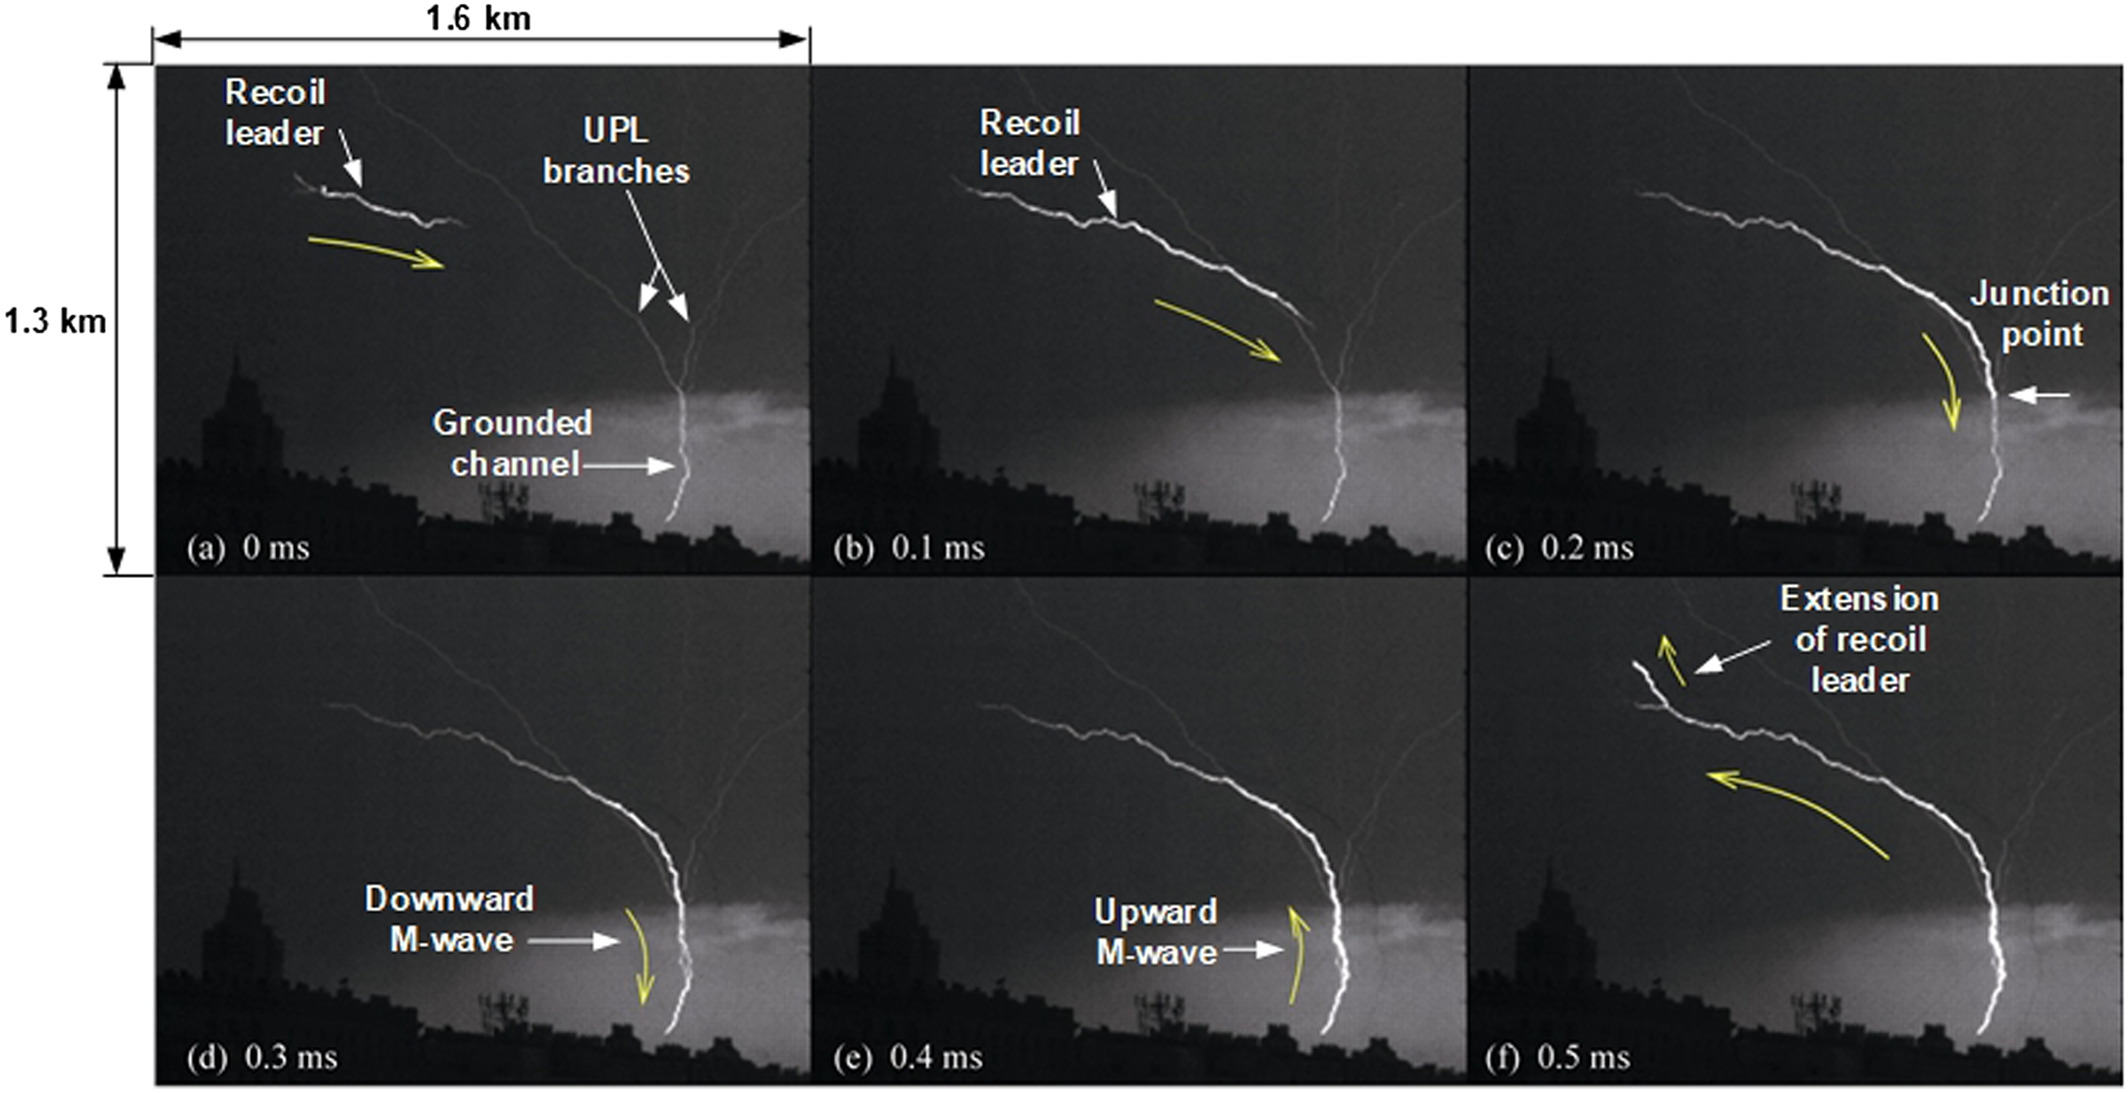
\includegraphics[width=\textwidth]{imagens/processo_componente_m.jpg}
		\caption{Evidência óptica do mecanismo da componente M de onda-guiada exibido por um pulso inicial de corrente contínua ascendente de um relâmpago negativo iniciado a partir de uma torre de 112 m. Mostradas nas figuras (a) a (f) estão seis quadros consecutivos separados por 100 $\mu s$, nos quais é possível observar um líder de recuo em um ramo decadente de um líder positivo ascendente que faz conexão com o canal aterrado e portador de corrente e inicia uma onda M descendente ao longo desse canal, do ponto de junção à ponta da torre, seguida por uma onda M ascendente refletida no solo que refaz e estende o canal do líder de recuo. Adaptado de Jiang et al. (2014)}
		\label{Component_M_explained}
	\end{figure}
	
	
	\pagebreak
	\section{Referências}
	\begin{thebibliography}{99}
		\bibitem{RAKOV_UHMAN} Rakov, V., \& Uman, M. (2007). Lightning: Physics and Effects. Cambridge University Press.		
		\bibitem{UHMAN_1987}  Uman, M A. The lightning discharge. United States: N. p., 1987. Web. 
		\bibitem{TRAN_2019}  Tran, M. D., \& Rakov, V. A. (2019). An advanced model of lightning M-component. Journal of Geophysical Research: Atmospheres, 124, 2296– 2317. https://doi.org/10.1029/2018JD029604 
		\bibitem{IUDIN_2015} D. I. Iudin and S. S. Davydenko (2015). FRACTAL MODEL OF A COMPACT INTRACLOUD DISCHARGE. I. FEATURES OF THE STRUCTURE AND EVOLUTION.
	\end{thebibliography}

\end{document}